\section{FIGHTING AS AN ELEMENT}

\begin{figure}[htbp]
    \centering
    \begin{tikzpicture}[figstyle]

        % coordinates
        \coordinate (naked_start) at (5,0);
        \coordinate (spiked_start) at (-5,0);
        \coordinate (bandit) at (0,70);

        \coordinate (naked_notch_start) at (5,25);
        \coordinate (spiked_notch_start) at (-5,25);

        % bandit wez
        \draw[fill=red!40]
            (bandit)
            -- ++(-60:15)
            arc (-60:-120:15)
            -- (bandit);
        
        % timeline
        \draw[->] 
            (naked_start) -- 
            node[below, pos=0]{
                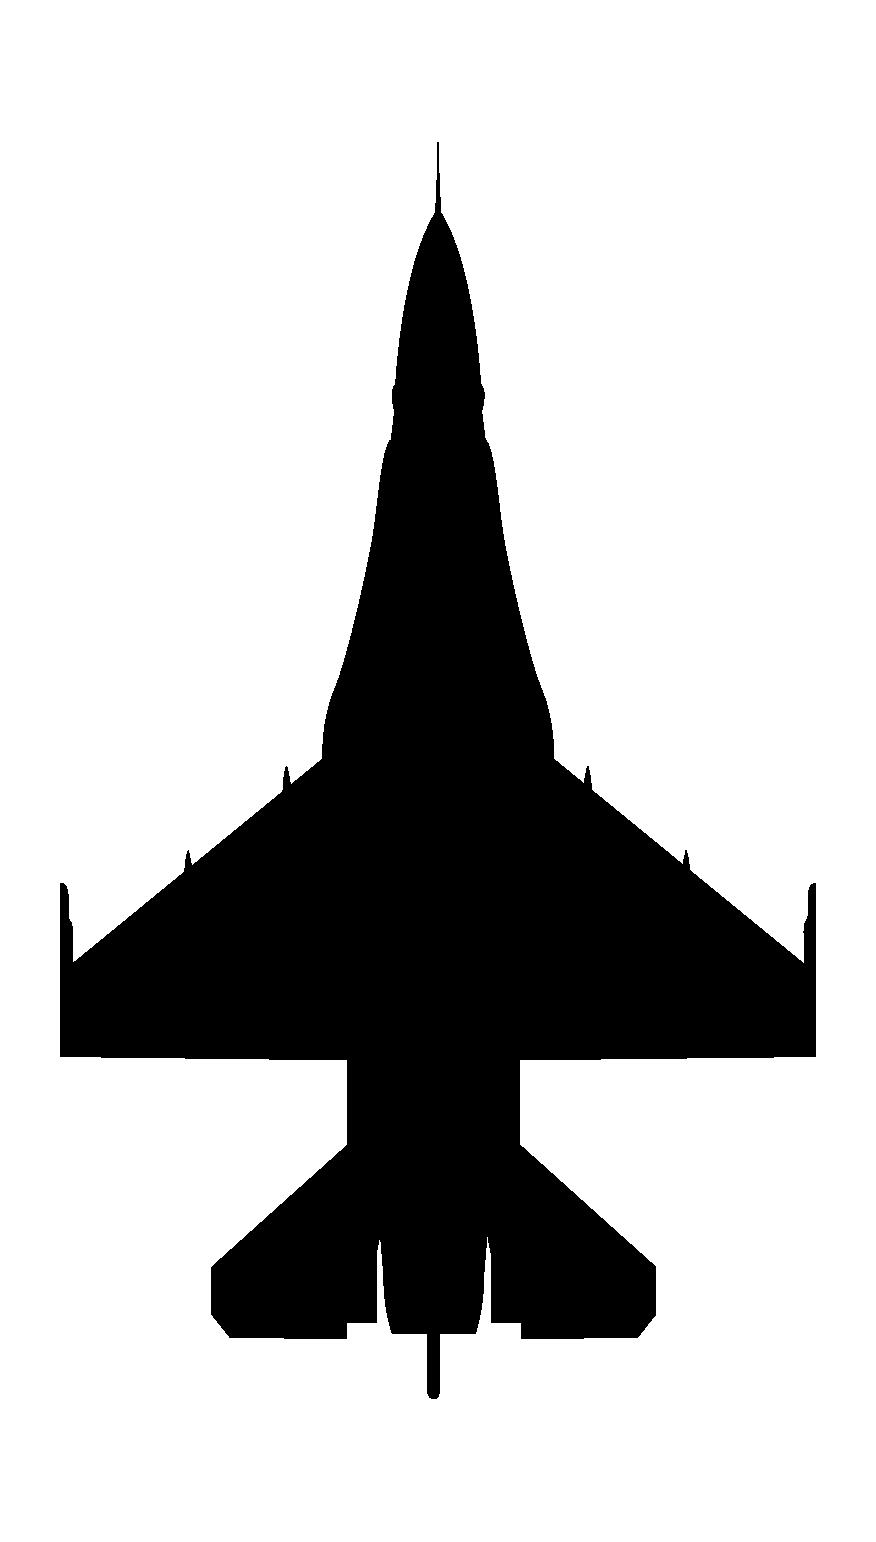
\includegraphics[
                width=7.5mm,
            ]{diagrams/aircraft/silhouette_f16_top.pdf}} 
            (naked_notch_start);
        \draw[->]
            (naked_notch_start)
            arc (180:90:5) 
            -- ++(10,0)
            arc (-90:0:5) 
            -- ++(0,10)
            node[above, pos=1]{
                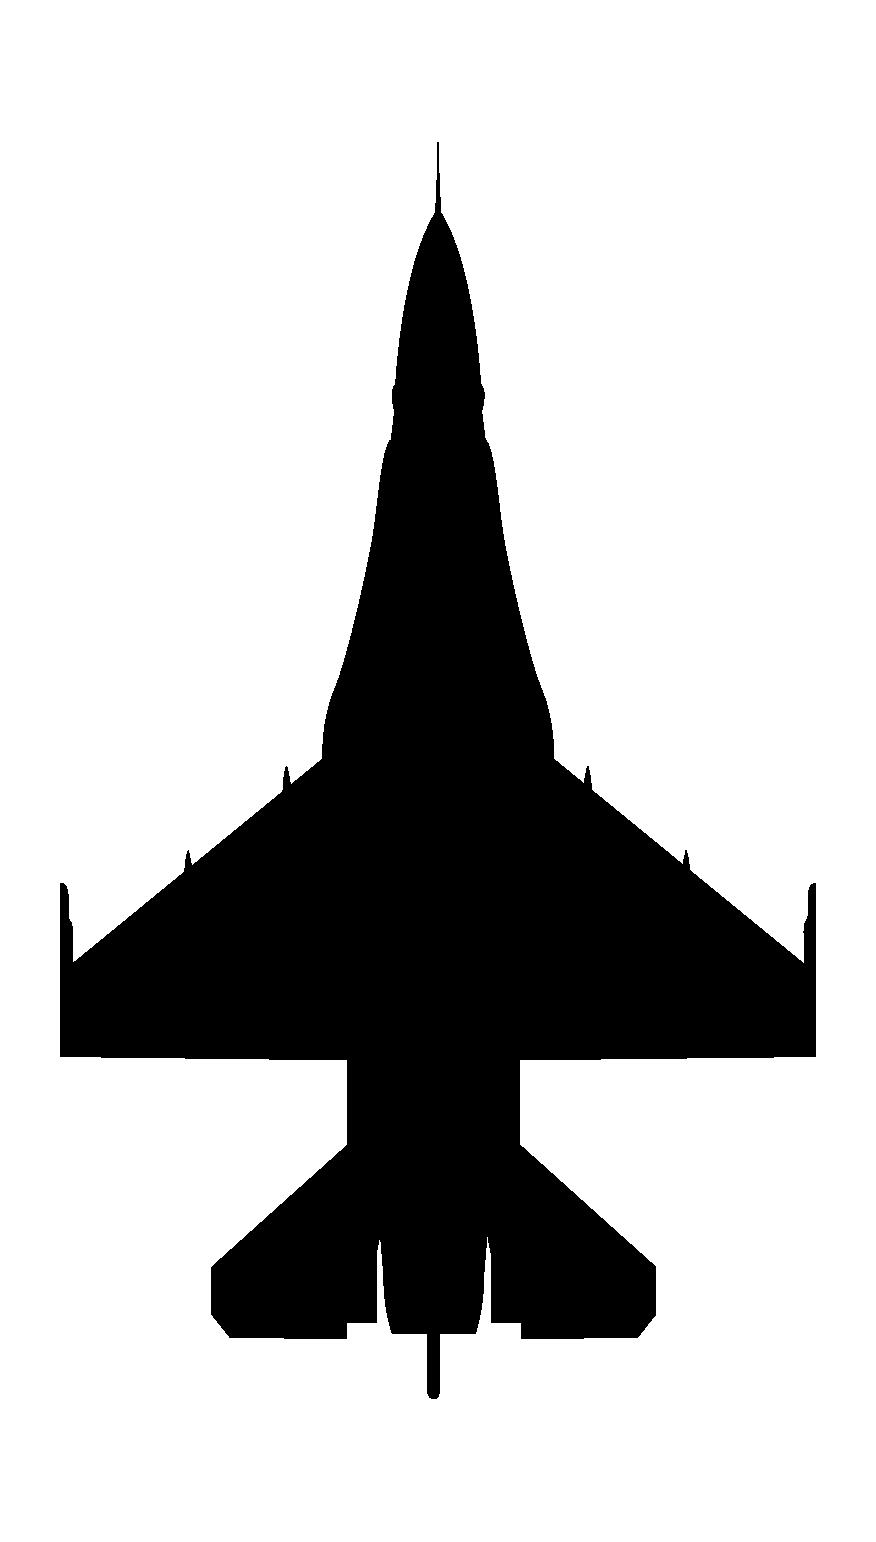
\includegraphics[
                    angle=0,
                    width=7.5mm,
            ]{diagrams/aircraft/silhouette_f16_top.pdf}};
        \draw[->] 
            (spiked_start) -- 
            node[below, pos=0]{
                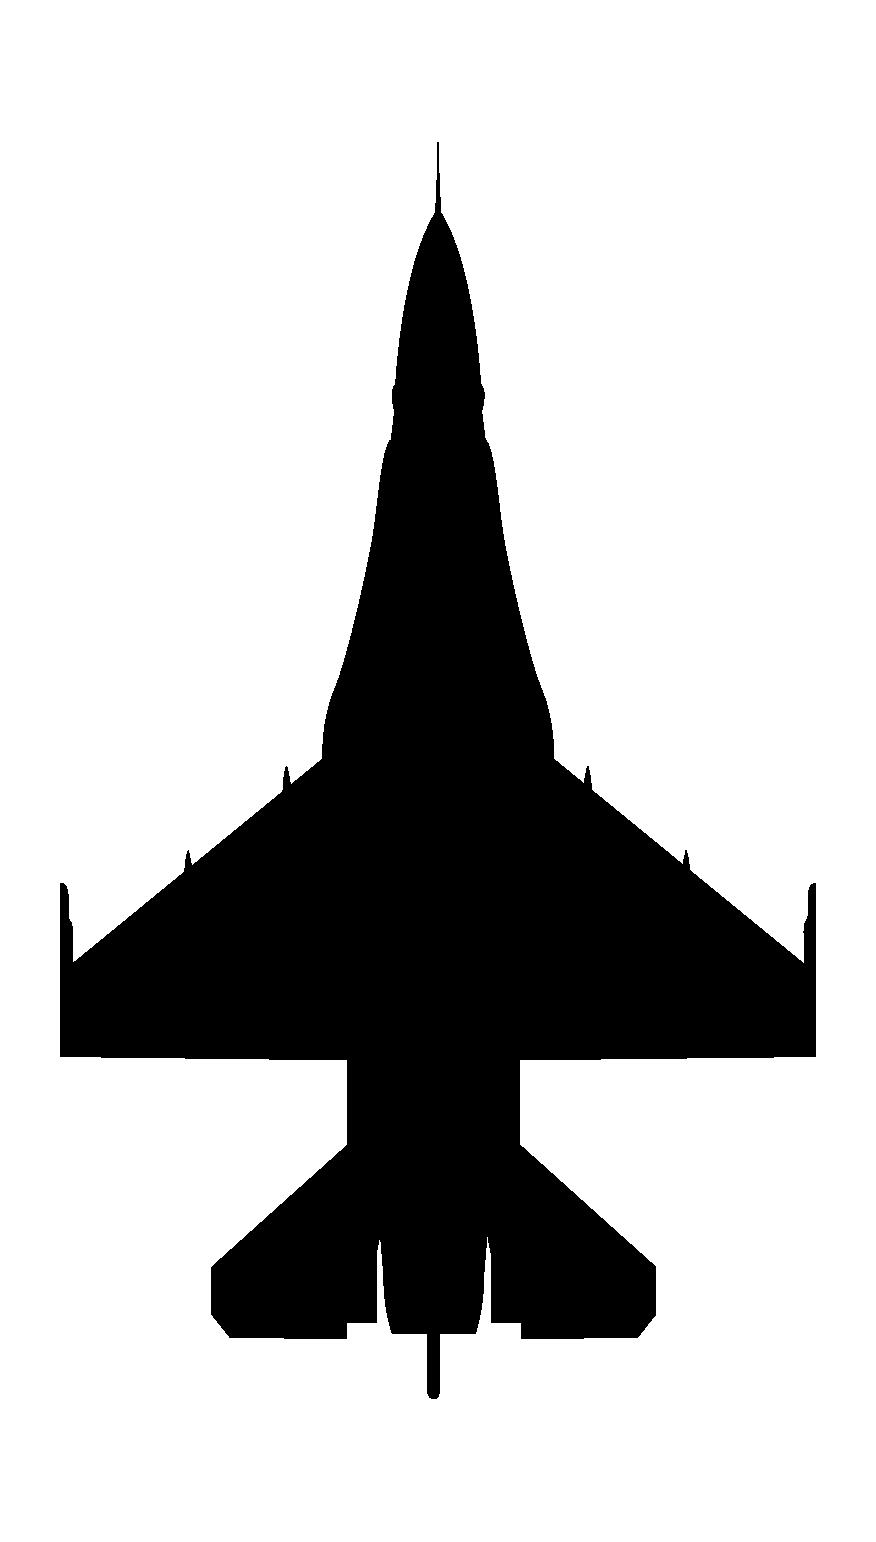
\includegraphics[
                width=7.5mm,
            ]{diagrams/aircraft/silhouette_f16_top.pdf}} 
            (spiked_notch_start);
        \draw[->]
            (spiked_notch_start)
            arc (0:90:5) 
            -- ++(-10,0)
            arc (90:180:5) 
            -- ++(0,-10)
            node[below, pos=1, ]{
                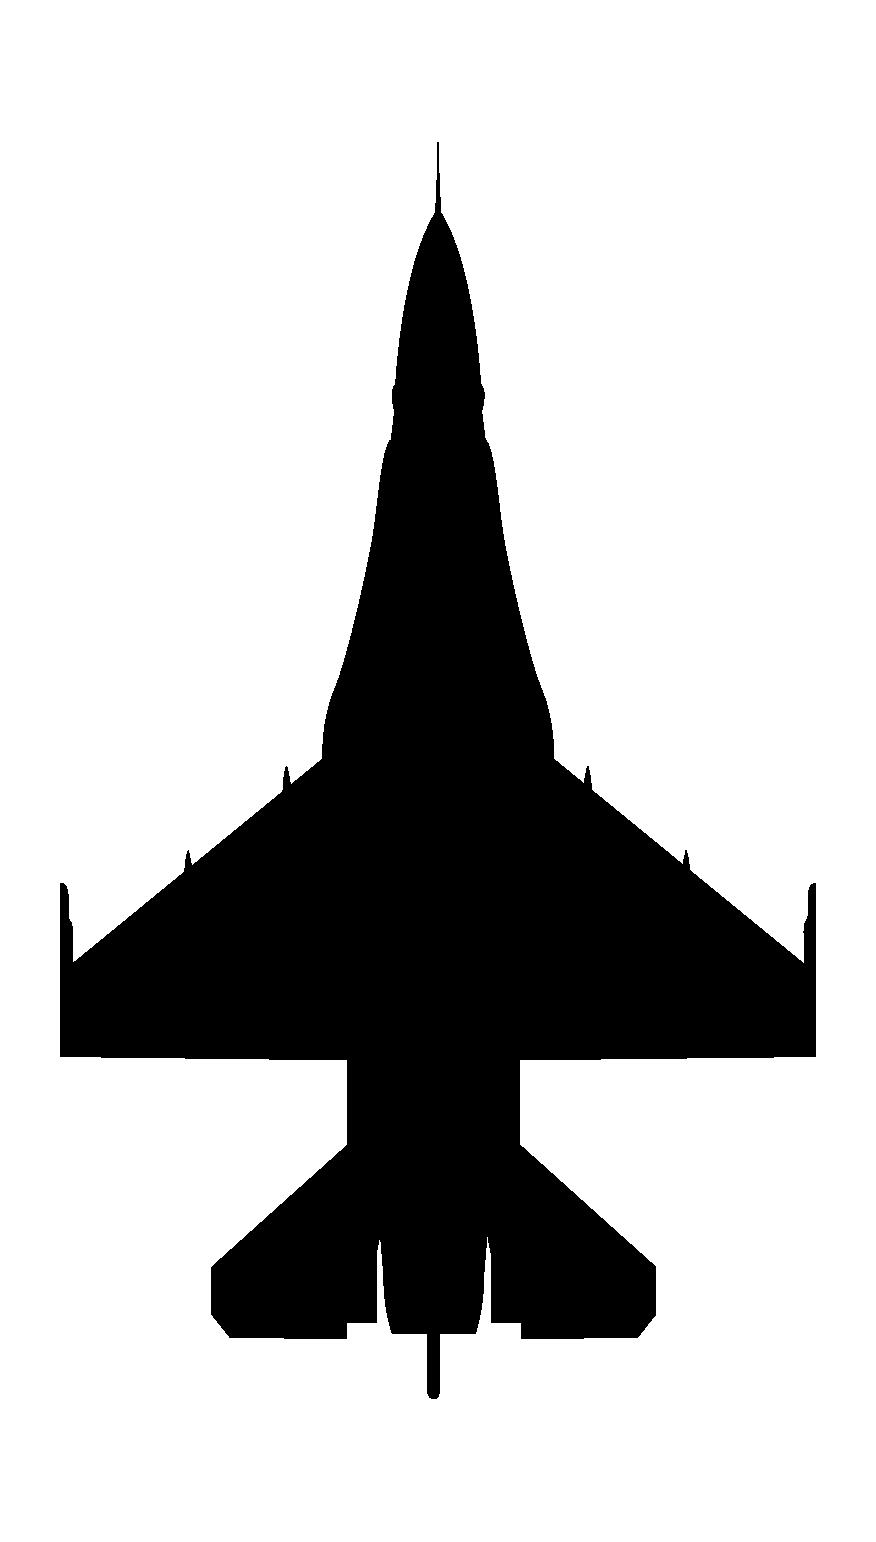
\includegraphics[
                    angle=180,
                    width=7.5mm,
            ]{diagrams/aircraft/silhouette_f16_top.pdf}};

        % bandit
        \node[] at (bandit) {
            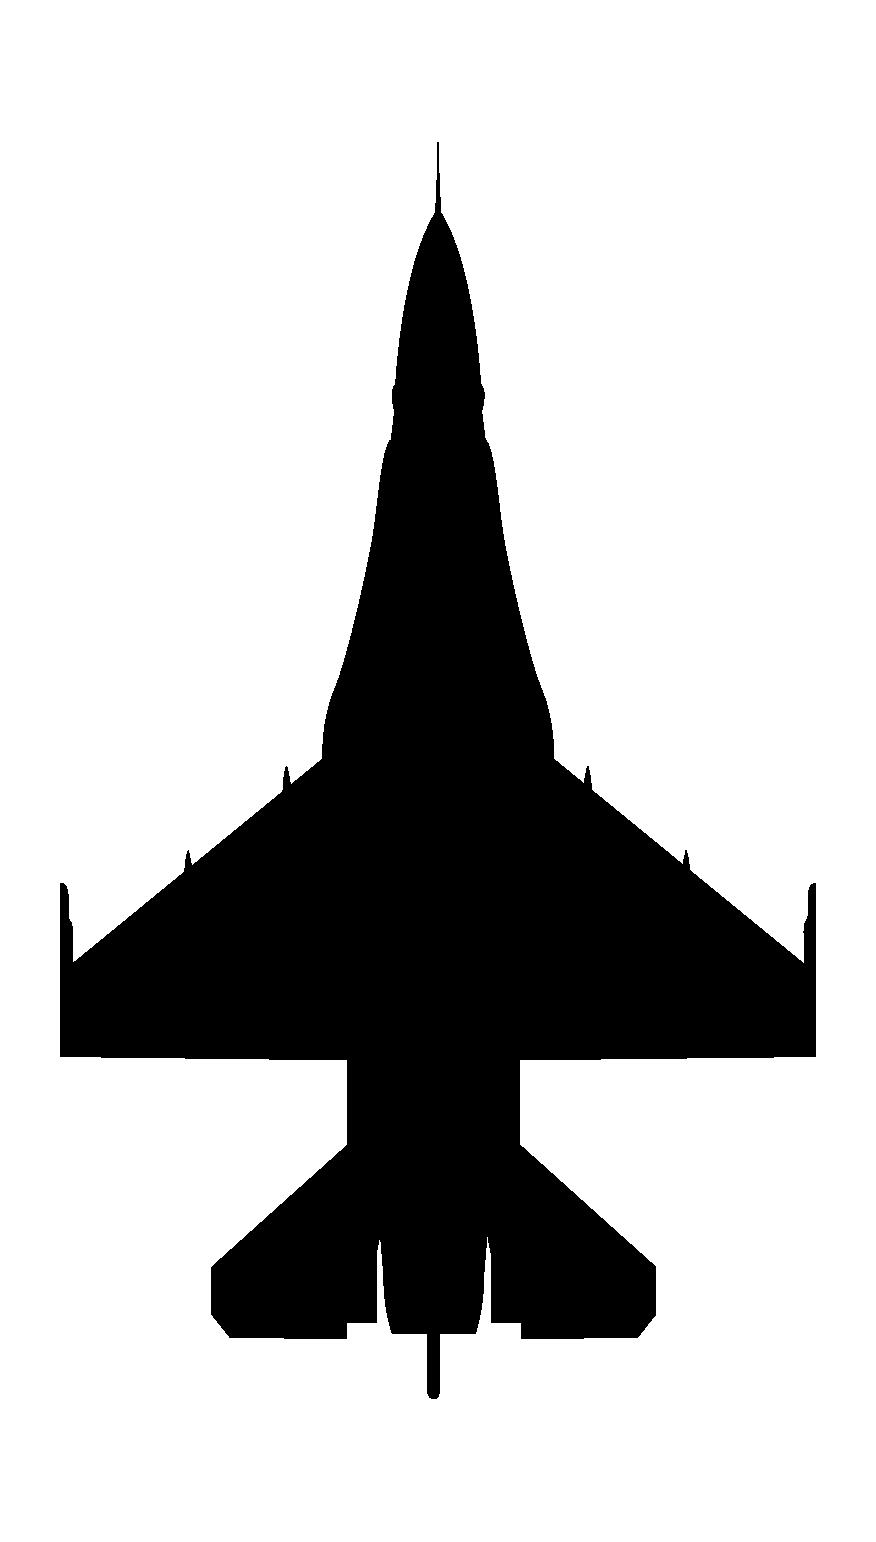
\includegraphics[
                angle=180,
                width=7.5mm,
        ]{diagrams/aircraft/silhouette_f16_top.pdf}};

    \end{tikzpicture}
    \caption{Banzai timeline}
    \label{fig:ttp_aa:element}
\end{figure}